\documentclass{report}

% Paquetes y configuraciones adicionales
\usepackage{graphicx}
\usepackage[export]{adjustbox}
\usepackage{caption}
\usepackage{float}
\usepackage{titlesec}
\usepackage{geometry}
\usepackage{hyperref}

% Configura los márgenes
\geometry{
    left=2cm,   % Ajusta este valor al margen izquierdo deseado
    right=2cm,  % Ajusta este valor al margen derecho deseado
    top=3cm,
    bottom=3cm,
}

% Configuración de los títulos de las secciones
\titlespacing{\section}{0pt}{\parskip}{\parskip}
\titlespacing{\subsection}{0pt}{\parskip}{\parskip}
\titlespacing{\subsubsection}{0pt}{\parskip}{\parskip}


\begin{document}
	
	% Portada del informe
	
	\title{Despliegue de una aplicación MEAN en el IaaS de la ULL}
	\author{Samuel Martín Morales}
	\date{\today}
	
	\maketitle
	
	% Índice
	\tableofcontents
	
	% Secciones del informe
	\chapter{Introducción}
  Para esta tercera práctica de la asignatura \emph{Sistemas y Tecnologías Web}, se solicita el despliegue de una aplicación MEAN que permite comprobar la estructura de servidores que ha sido implementada en prácticas anteriores de la asignatura. 
  
  Tras esto, se solicita la creación de un nuevo servidor backend que se trate de una copia o de un clon del servidor backend que existía de manera previa en la infraestructura implantada. 
  
  Finalmente, tras la realización de estos pasos anteriores, se pide configurar la infraestructura para que el servidor \emph{Nginx} pueda realizar un balanceo de carga de las peticiones realizadas hacia dicho servidor Proxy, el cúal se encargará de realizar la distribución de las peticiones entre los dos servidores backend que existen en la infraestructura, permitiendo por tanto, un balanceo de carga.
	
	\chapter{Despliegue de una aplicación MEAN de prueba}
	Para el despliegue de una aplicación MEAN para la comprobación de la infraestructura implantada en prácticas anteriores, se hace uso de la siguiente \href{https://github.com/mongodb-developer/mean-stack-example}{aplicación} de prueba. Dicha aplicación, necesita del cambio de ciertos aspectos para que se pueda ejecutar de manera correcta en nuestra infraestructura.

  Pero, antes de comenzar con los cambios necesarios dentro del código de la aplicación clonada, se debe de realizar la configuración de la máquina backend, para que, permita que \emph{Visual Studio Code} pueda abrir la carpeta que contiene los distintos ficheros de la aplicación, dentro de la máquina virtual que se encuentra alojada en el IaaS de la ULL. 
  
  En un comienzo, se obtiene la clave rsa que se encuentra dentro de nuestra máquina personal, para poder realizar la conexión SSH con la máquina virtual que se encuentra alojada en el IaaS de la ULL. Para ello, se ejecuta el siguiente comando:

  \begin{verbatim}
    ssh-keygen -t rsa -b 4096 -C "
    samuel.martin.morales@estudiante.
    ull.es"
  \end{verbatim}

  A continuación, se accede a la máquina virtual la cúal se quiere configurar para que permita la conexión SSH desde la máquina personal, y se ejecutan los siguientes comandos:

  \begin{verbatim}
    mkdir ~/.ssh
    touch authorized_keys
    sudo nano authorized_keys
  \end{verbatim}

  Dentro de dicho fichero denominado como \emph{authorized\_keys}, añadimos la clave rsa generada de manera previa dentro de la máquina personal, y, tras todo esto ya se puede realizar la conexión de la máquina virtual con visual studio code para poder editar código dentro de este. Todo esto comentado anteriormente, queda reflejado en la siguiente imagen \ref{fig:Configuración-VSCode}.

  \begin{figure}[H]
    \centering
    \includegraphics[scale=0.5]{Capturas/Informe-P3-STW/Autorización-de-VS-para-poder-editar-código.png}
    \caption{Configuración de la máquina virtual para que se pueda editar código haciendo uso de Visual Studio Code.}
    \label{fig:Configuración-VSCode}
  \end{figure}
	
  Una vez configurado Visual Studio Code para poder editar el código necesario, se realiza la configuración del fichero \emph{.env} dentro del \emph{server} de la aplicación MEAN. Dentro de dicho fichero, se modifica el \emph{ATLAS-URI} existente, de tal manera que, permita conectarnos desde el server del backend hasta la base de datos implantada mediante \emph{MongoDB} dentro del servidor de base de datos que se ha instalado de manera previa en prácticas anteriores. Con todo esto anteior, se puede observar la siguiente imagen \ref{fig:Configuración-Fichero-env}.

  \begin{figure}[H]
    \centering
    \includegraphics[scale=0.8]{Capturas/Informe-P3-STW/Configuración-atlas-URI.png}
    \caption{Configuración del fichero .env.}
    \label{fig:Configuración-Fichero-env}
  \end{figure}

  Como se puede observar en la variable de entorno \emph{ATLAS-URI}, la estructura de la ruta es la siguiente:

  \begin{verbatim}
    mongodb://mongodb://<username>:<password>@<ip_direction>:<port>/<database_name>
  \end{verbatim}

  Otra de las configuraciones que se deben de hacer para la correcta ejecución de la aplicación MEAN suministrada, se produce dentro del fichero denominado \emph{package.json} dentro del cliente de la aplicación. En este fichero, se debe de configurar uno de los scripts de inicio del cliente, de tal manera que, se encuentre escuchando la interfaz de red de nuestro servidor backend, de forma que, cuando el servidor Proxy realice un \emph{Proxy\_Pass} hacia el servidor backend, este pueda escuchar las peticiones que se le realizan desde el servidor Proxy. Con todo esto comentado, se puede observar la siguiente imagen \ref{fig:Configuración-script-client} dónde se muestra la correcta configuración del script de inicio del cliente de la aplicación MEAN, de manera que funcione para la infraestructura implementada.

  \begin{figure}[H]
    \centering
    \includegraphics[scale=0.8]{Capturas/Informe-P3-STW/Configuración-ng-serve.png}
    \caption{Configuración del script de inicio del cliente.}
    \label{fig:Configuración-script-client}
  \end{figure}

  Tras estas configuraciones realizadas, se puede iniciar la instalación de las dependencias necesarias:

  \begin{verbatim}
    npm install
  \end{verbatim}

  Una vez instaladas las dependencias necesarias, se puede iniciar la aplicación MEAN de prueba, para ello, se ejecuta el siguiente comando:

  \begin{verbatim}
    npm start
  \end{verbatim}

  Finalmente, se puede observar el correcto funcionamiento de la aplicación MEAN de prueba, en las siguientes imágenes \ref{fig:Funcionamiento-1}, \ref{fig:Funcionamiento-2}.

  \begin{figure}[H]
    \centering
    \includegraphics[scale=0.4]{Capturas/Informe-P3-STW/Ejecución-aplicación-MEAN-en-terminal.png}
    \caption{Funcionamiento de la aplicación MEAN de prueba dentro de la terminal de la máquina Backend.}
    \label{fig:Funcionamiento-1}
  \end{figure}

  \begin{figure}[H]
    \raggedright
    \includegraphics[scale=0.3]{Capturas/Informe-P3-STW/Funcionamiento-aplicación-MEAN.jpg}
    \caption{Funcionamiento de la aplicación MEAN, desde cualquier navegador.}
    \label{fig:Funcionamiento-2}
  \end{figure}

	\chapter{Clonado de la máquina virtual Backend}
  Una vez se ha comprobado el correcto funcionamiento de la infraestructura implantada en prácticas anteriores gracias al despliegue de la aplicación MEAN de prueba, se procede a la clonación del servidor backend existente de manera previa en la infraestructura. Para ello, se realiza una copia de la máquina virtual que se encuentra alojada en el IaaS de la ULL, para ello, se observa en la siguiente imagen \ref{fig:Clonado-1} dónde se puede ver la nueva estructura de la infraestructura, junto con el establecimiento de la distintas direcciones ip que van a ser instauradas dentro de las distintas interfaces de red de dicha máquina.

  \begin{figure}[H]
    \centering
    \includegraphics[scale=0.7]{Capturas/Informe-P3-STW/Estructura-nueva-configuración-servicio.png}
    \caption{Estructura de la nueva configuración de infraestructura.}
    \label{fig:Clonado-1}
  \end{figure}

  Teniendo en cuenta todo esto anterior, se realiza la creación de la nueva máquina virtual, la cuál, poseerá dos nuevas interfaces de red, una de ellas correspondiente con la \emph{DOCINT4 (172.16.14.77/172.16.14.78)} y la \emph{DOCINT3 (172.16.15.77/172.16.15.78)}. Antendiendo a esto, se puede observar el siguiente fichero de configuración de interfaces \ref{fig:Clonado-2} y la comprobación del funcionamiento de las interfaces de red de la nueva máquina clonada \ref{fig:Clonado-3} y \ref{fig:Clonado-4}.

  \begin{figure}[H]
    \centering
    \includegraphics[scale=0.5]{Capturas/Informe-P3-STW/Configuración-interfaces-nuevo-servidor-backend.png}
    \caption{Configuración de interfaces de red de la nueva máquina clonada.}
    \label{fig:Clonado-2}
  \end{figure}

  \begin{figure}[H]
    \centering
    \includegraphics[scale=0.5]{Capturas/Informe-P3-STW/Comprobación-funcionamiento-nueva-interfaz-backend.png}
    \caption{Comprobación del funcionamiento de las interfaces de red de la nueva máquina clonada.}
    \label{fig:Clonado-3}
  \end{figure}

  \begin{figure}[H]
    \raggedright
    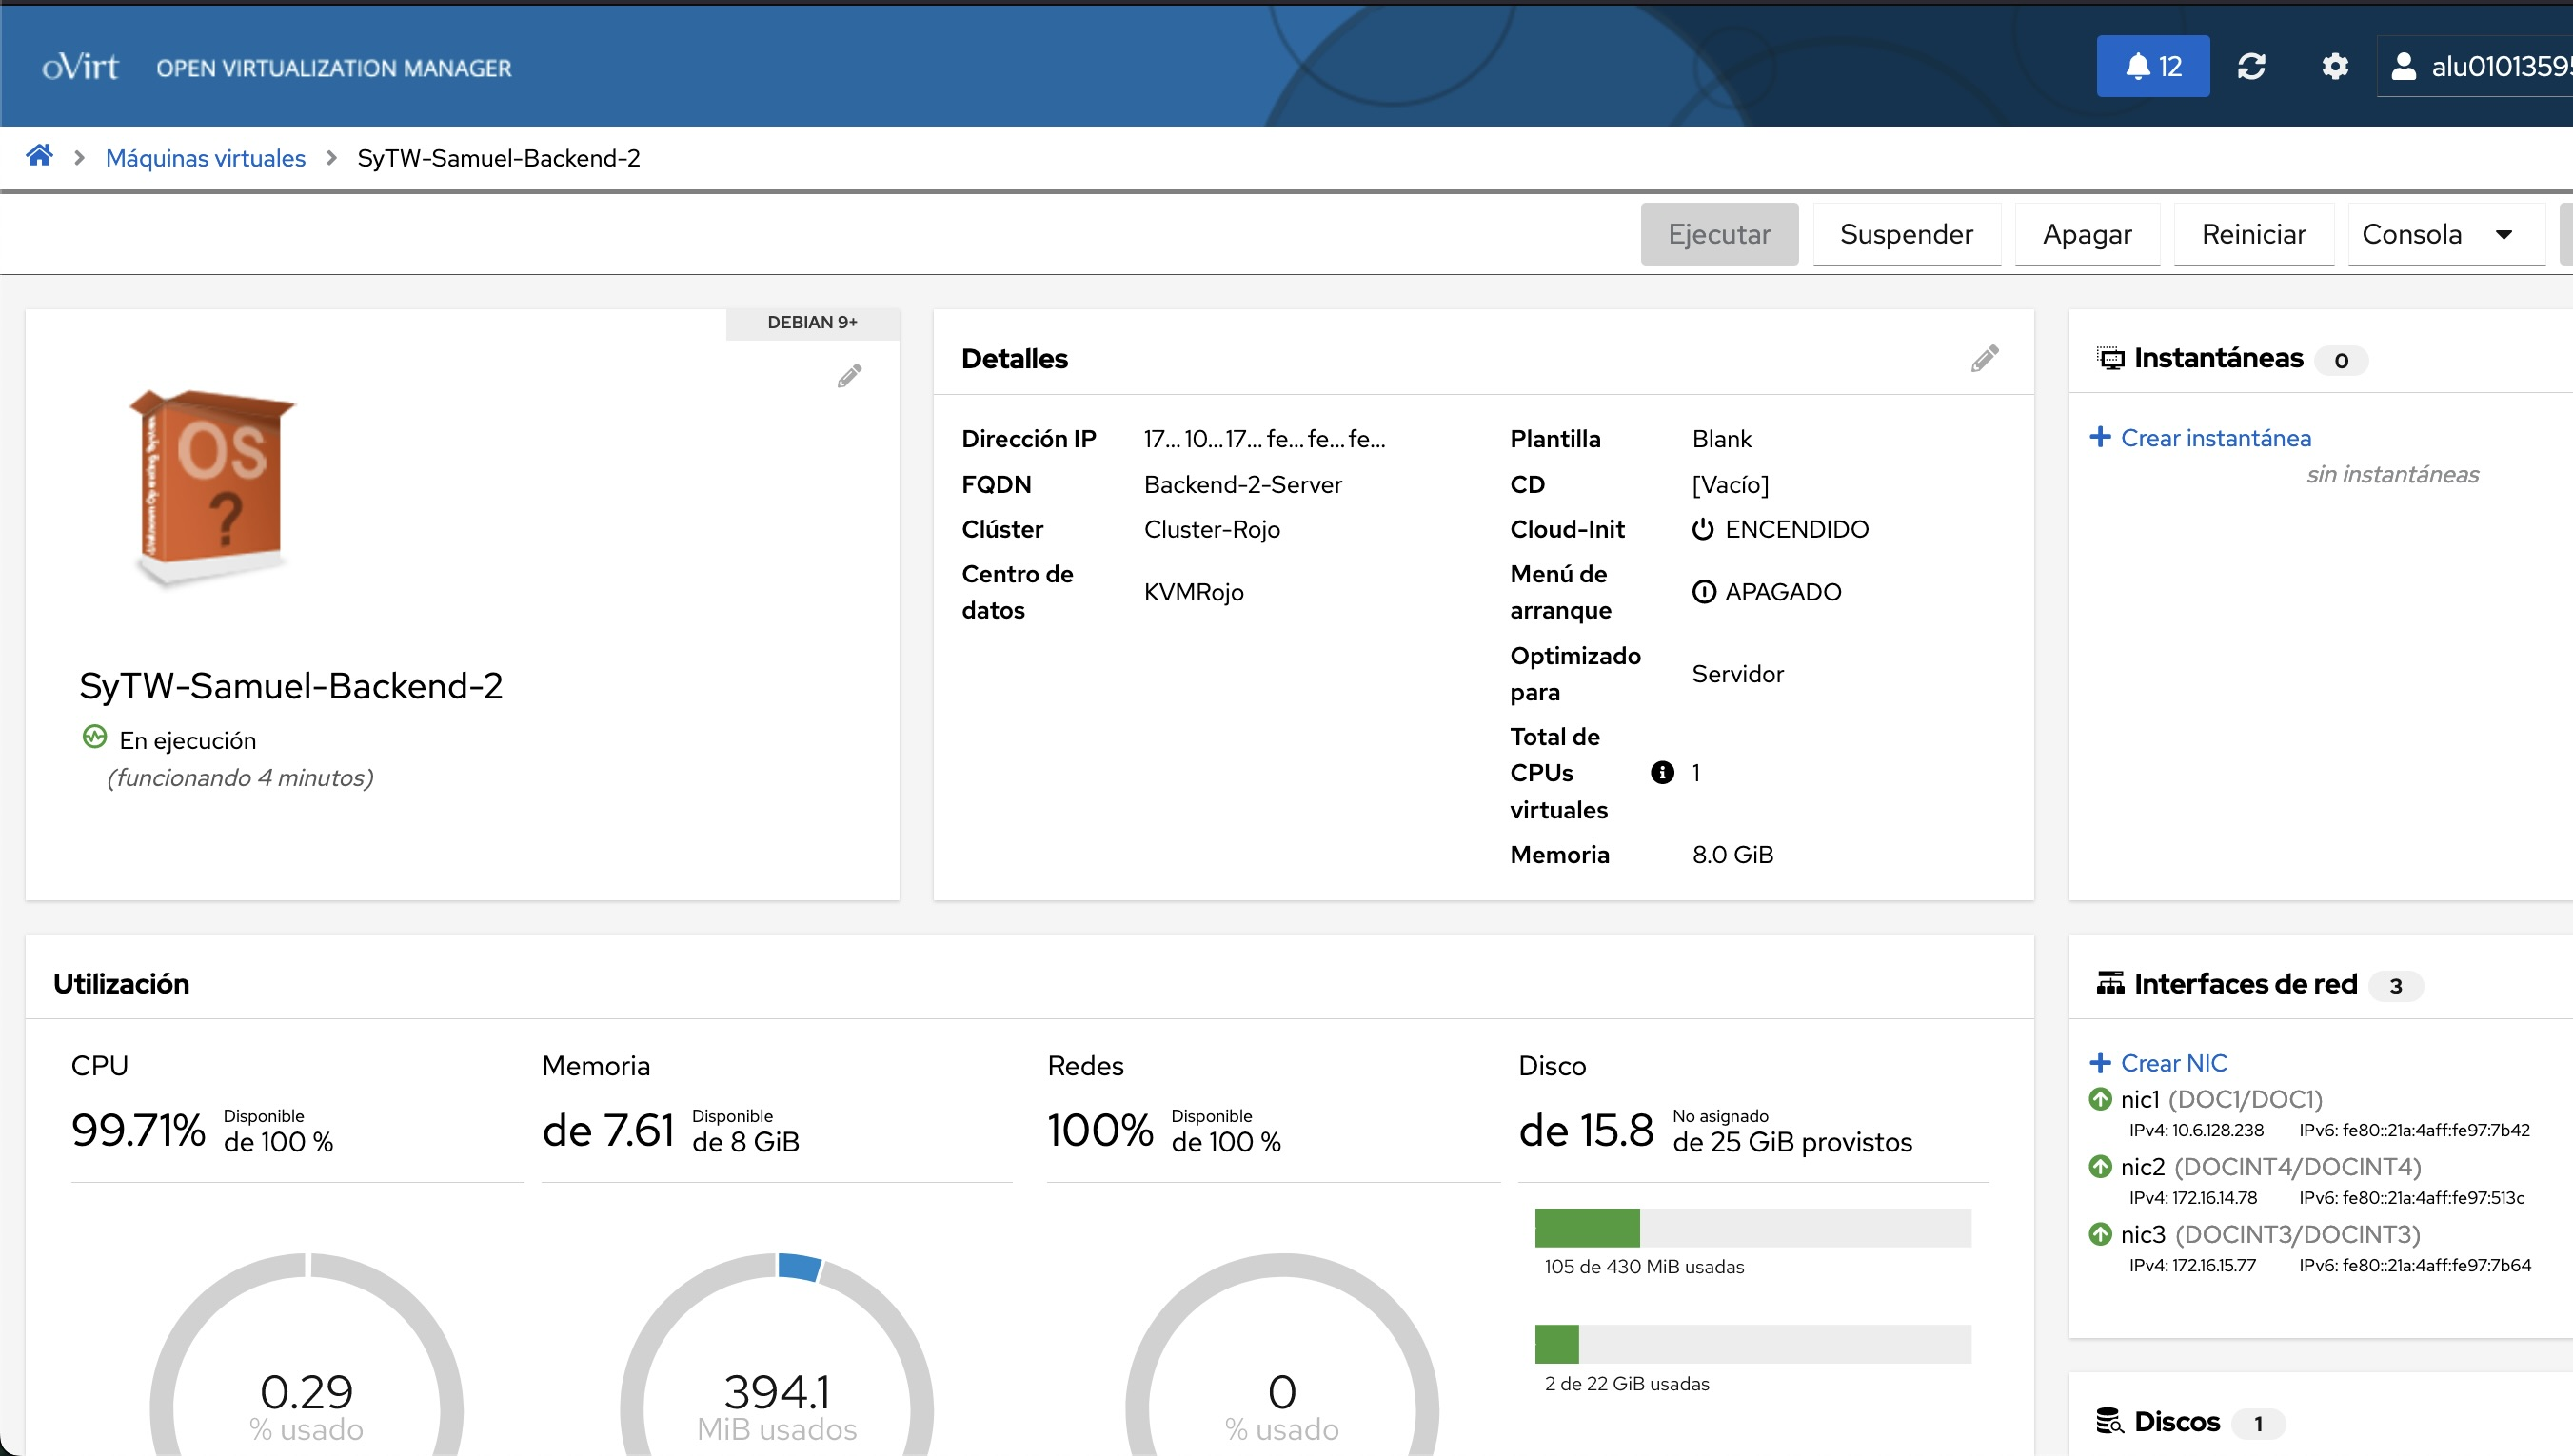
\includegraphics[scale=0.4]{Capturas/Informe-P3-STW/Nuevo-servidor-backend.jpeg}
    \caption{Comprobación del funcionamiento de las interfaces de red de la nueva máquina clonada.}
    \label{fig:Clonado-4}
  \end{figure}

  Finalmente, tras la configuración de manera correcta de las distintas interfaces de red de la nueva máquina clonada, se procede a la instalación de los distintos paquetes que fueron instalados de manera previa, para ello, se puede visualizar el informe de la práctica \href{https://drive.google.com/file/d/1hmTNhYU0AJ1pRHuNVUaLL7Eal5yHOkge/view?usp=drive_link}{2} de la asignatura \emph{Sistemas y Tecnologías Web}.

  \chapter{Configuración del Proxy como sistema de balanceo de carga}
  Una vez se ha realizado la clonación de la máquina virtual que se encuentra alojada en el IaaS de la ULL, se procede a la configuración del servidor Proxy para que este pueda realizar un balanceo de carga entre los dos servidores backend que existen en la nueva infraestructura. Para ello, se realiza la configuración de \emph{Nginx}, de manera que pueda redistribuir peticiones entre los dos servidores backend que existen en esta.

  En este caso, se configura el fichero \emph{default}, de manera que pueda realizar el balanceo de la carga de forma que el doble de las peticiones irá para el servidor backend con interfaz de red \emph{172.16.12.78}, mientras que el otro servidor backend con interfaz de red \emph{172.16.14.78} tendrá un peso de 1.

  Todo esto comentado anteriormente, se puede observar en la siguiente configuración del fichero de configuración \emph{default} de \emph{Nginx} \ref{fig:Configuración-Nginx}.

  \begin{figure}[H]
    \centering
    \includegraphics[scale=0.4]{Capturas/Informe-P3-STW/Configuración-fichero-nginx-para-balanceo-de-carga.png}
    \caption{Configuración del fichero default de Nginx para la implementaciñon del sistema de balanceo de carga.}
    \label{fig:Configuración-Nginx}
  \end{figure}

  \chapter{Conclusión}
  Para finalizar, se puede concluir que la realización de esta práctica ha sido de gran utilidad para poder comprender el funcionamiento de un sistema de balanceo de carga, así como la configuración de un servidor Proxy para que este pueda realizar un balanceo de carga entre los distintos servidores backend que existen en la infraestructura. Además, se ha podido comprobar el correcto funcionamiento de la infraestructura implantada en prácticas anteriores, gracias al despliegue de una aplicación MEAN de prueba. Es por ello que, esta tercera práctica de la asignatura me ha servido como aprendizaje para poder buscarme la vida para comprender el funcionamiento del código y de la aplicación implantada por otro programador como es la aplicación MEAN usada para la comprobación del funcionamiento de la infraestructura. 

  Para finalizar, el establecimiento de un sistema de balanceo de carga también me permite comprender un poco más sobre cómo funciona de manera real las infraestructuras de servidores que se encuentran en la actualidad, ya que, en la mayoría de los casos, se suele implementar un sistema de balanceo de carga entre los distintos servidores backend que existen, de manera que se pueda realizar una distribución de las peticiones que se realizan hacia el servidor Proxy, entre los distintos servidores de la infraestructura, permitiendo por tanto, un balanceo de carga.
	
\end{document}